
\chapwithtoc{Introduction}
\label{sec:Introduction}

\lsystem (also called Lindenmayer system) is mathematical formalism developed for plant growth modeling by Aristid Lindenmayer in 1968~\cite{Lin68}.
An example of plant modeled by \lsystem is in \autoref{fig:introLilac}.
In the simplest form an \lsystem is variant of regular or \mbox{context-free} grammar.
By rewriting (deriving) initial string of symbols (also called axiom) with rewrite rules from grammar \lsystem produces string of symbols which can be interpreted in many different ways.
In first \lsystems by Lindenmayer were symbols interpreted as cells of algae.
A different approach was taken by Przemyslaw Prusinkiewicz who interpreted \lsystem symbols with \mbox{Logo-like} turtle\footnote{
	Logo is computer programming language developed for use in education of programming for children.
	Logo controls cybernetic turtle which is drawing on 2D canvas.}~\cite{Pru85}.
With this method he obtained more plant-like structures and fractals~\cite{CD93}.
In \autoref{fig:introHTree} you can see H-tree fractal created by \lsystem.

\begin{figure}[ht]
	\centering
	\subfloat[Model of lilac panicle]{
		\includegraphics[width=0.48\textwidth]{lilac}
		\label{fig:introLilac}
	} ~
	\subfloat[H-tree fractal]{
		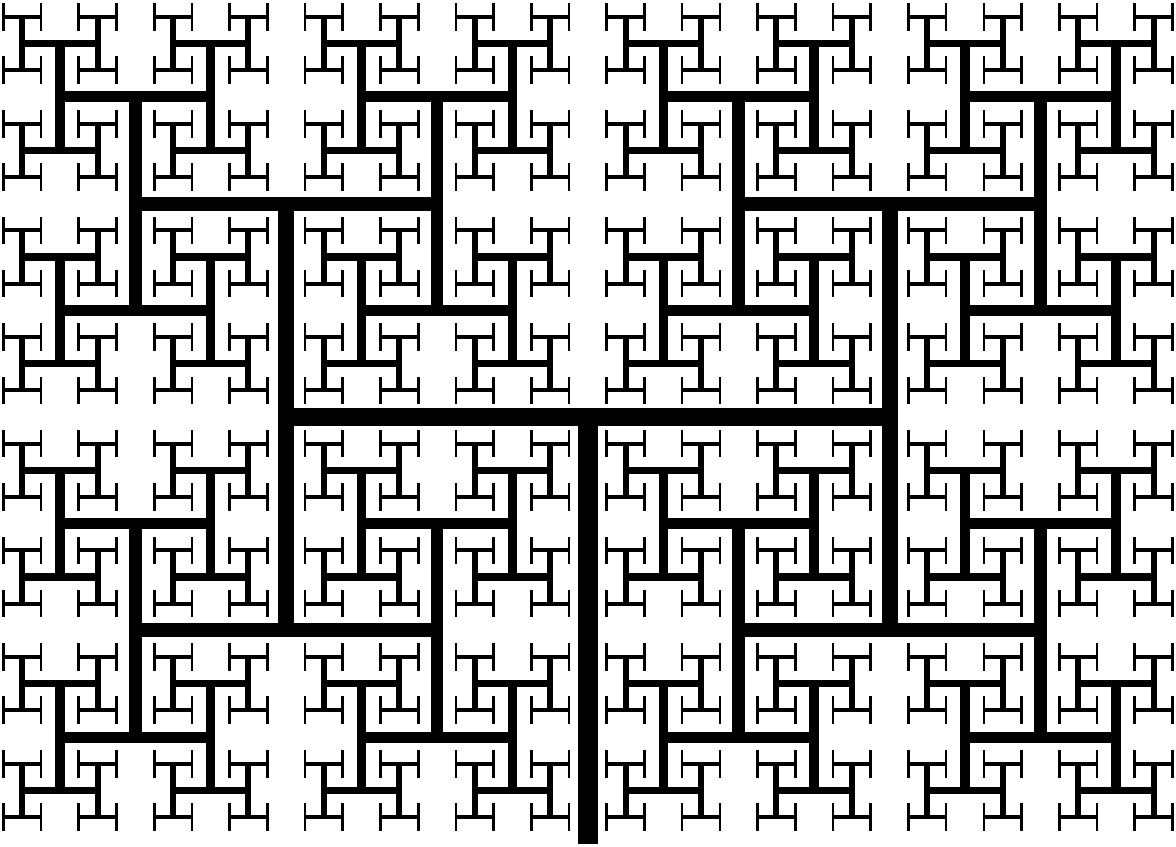
\includegraphics[width=0.48\textwidth]{HTree}
		\label{fig:introHTree}
	}
	\caption{Examples of models created by \lsystem}
\end{figure}


Over the time \lsystems were used in many areas.
For example they were used to generate rivers in fractal mountains~\cite{PH93}, streets in virtual cities~\cite{PM01} and to describe subdivision of curves~\cite{PSSK03}.
\lsystems can be used in other fields than computer graphics for example in music generation~\cite{HCJ99, Man06}.
They are still used in plant modeling.
Plant models generated with \lsystems are used in modern video games or films, for example they were used to generate many plants and trees for famous film Avatar~\cite{Wor08, Dun10}.~\footnote{\citeauthor{SBM10} presented reverse method -- automatic generation of \lsystems from 2D model~\cite{SBM10}.}

\lsystems has wide variety of interesting applications but it is hard to find some place to experiment with them.
There are two base types of \lsystem generators, web-based and desktop applications.
Web-based \lsystem generators are easily accessible but they are often too primitive and do not offer nothing more than generation of simple fractals (see \autoref{sec:WebBasedGenerators}).
Some of them do not work in the most used browsers.

Desktop applications generally offers more options than web-based but most of them is also quite simple and do not offer advanced features of \lsystems.
There are some complex applications that offers pretty good features but there are not free, it is hard to control them or they are old and not maintained (see \autoref{sec:DesktopGenerators}).
Problem with desktop applications is also in compatibility with user's operating system, its version and installed libraries.

The main goal of this work is to take the good from both approaches and create online feature-rich development environment for anybody who wants to experiment with \lsystems.
Development environment will be divided into two parts, web user interface and \lsystem processing library.

\begin{wrapfigure}{r}{0.5\textwidth}
	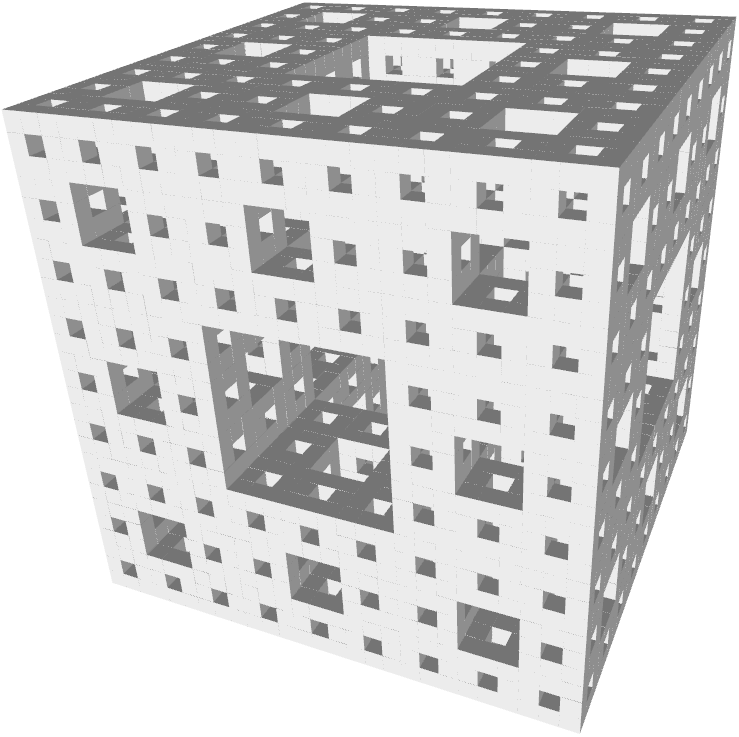
\includegraphics[width=\linewidth]{MengerSponge}
	\caption{Menger sponge created by \lsystem}
	\label{fig:introMengerSponge}
\end{wrapfigure}

User interface will be web site which offers great accessibility.
Anybody around the world can use it from any device connected to the Internet like computers, laptops, tablets or smart phones.
Interface should be friendly to new users and also offer advanced features for experienced users.
Primary output format of web based \lsystem processor will be 2D images but it will also be possible to create and display 3D outputs using modern HTML5 WebGL\footnote{
	WebGL (Web-based Graphics Library) is a cross-platform, royalty-free web standard for a low-level 3D graphics API based on OpenGL ES 2.0, exposed through the HTML5 Canvas element as Document Object Model interfaces.
	WebGL code executes on a computer display card's GPU (Graphics Processing Unit).} technology directly in browser.
In \autoref{fig:introMengerSponge} is print-screen of Menger Sponge model displayed by WebGL.
Part of the web site will be gallery of \lsystems.
Any registered user can add his \lsystems to gallery along with some description and others can rate it.
This will help to create community of active users and it can also serve as learning tool for new users.

Second part of application will be \lsystem processing library.
Although it will be designed to support demands of web interface, it will be independent and it should be possible to use it in other application.
During design of library great emphasis will be placed on easy extensibility to make the it as universal as possible.
It will possible to extend library by user.

New syntax for input will be designed to improve user experience especially for new users.
The syntax should be clean, easy to understand and remember.
%The syntax will cover all needs of library from defining \lsystems to configuring whole processing system.
%This will also ensure that whole input can be written in one file which will simplify source code sharing and saving.
%Parser generator will be used for creating robust and extensible parser.


\section*{Structure of thesis}

In the first chapter \lsystems are formally defined and explained their rewriting and interpretation principles.
Follows is description of \lsystem types and their properties.
At the end on the first chapter is list of related \lsystem generators.

The second chapter is devoted to the ... [to be continued].

All source codes of \lsystems in this thesis are in designed syntax and it is possible to process them on the web.
Syntax reference can be found in Attachment \ref{chap:syntax}.
All figures of plants or fractals in this thesis (if not stated otherwise) are produced by created program.
More information about figures and their source codes is in Attachment \ref{chap:aboutFigures}.































